\chapter{Architettura Funzionale del Sistema Realizzato}	

\section{Struttura e funzionamento di YAFS}

Per le simulazioni realizzate nel corrente lavoro di Tesi è stato fatto uso del simulatore \textit{YAFS} \footnote{Disponibile su: \url{https://github.com/acsicuib/YAFS}} (\textit{Yet Another Fog Simulator}) \cite{YAFSSimulator}. Quest'ultimo utilizza una libreria per la generazione e la gestione degli eventi chiamata \textit{SimPy} \footnote{Disponibile su: \url{https://simpy.readthedocs.io}}. Simpy è un'implementazione di un simulatore ad eventi discreti (DES, \textit{Discrete Event Simulator}), che garantisce un'interfaccia per la definizione dei processi (i componenti attivi della simulazione) e delle risorse (ad esempio i nodi ed i collegamenti della rete).

YAFS è definito principalmente da sei classi: \textit{Core}, \textit{Topology}, \textit{Selection}, \textit{Placement}, \textit{Population} e \textit{Application}. Le relazioni che intercorrono tra loro sono mostrate in Figura \ref{fig:YAFS_classes}.

\begin{figure}[!ht]
  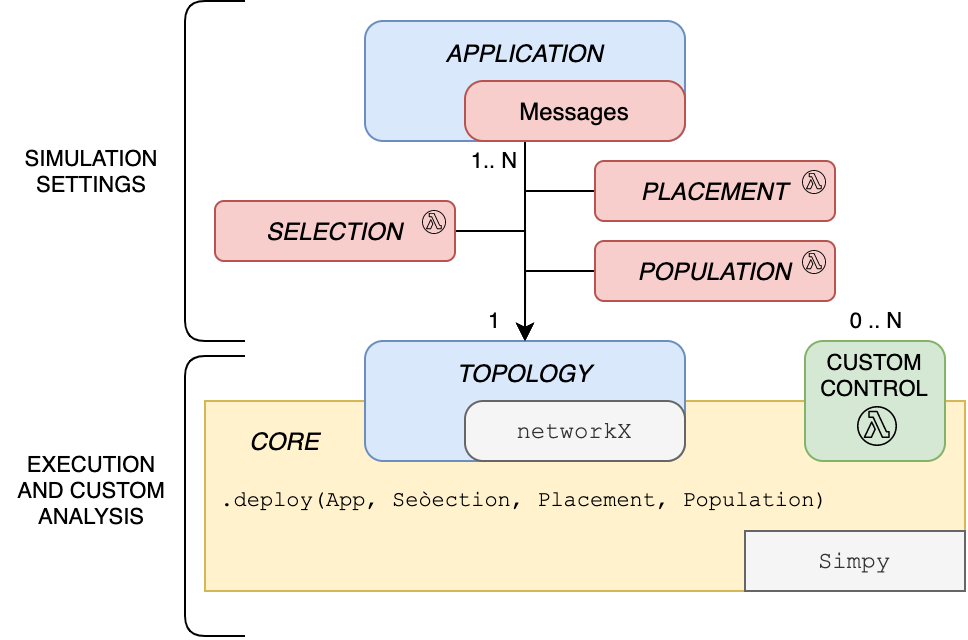
\includegraphics[width=12cm]{images/YAFS_classes}
  \centering
  \caption[Architettura di YAFS]{Architettura di YAFS}
  \label{fig:YAFS_classes}
\end{figure}

\subsection{Topologia e modellazione delle entità}

Le entità della topologia sono modellate come un insieme di \textit{nodi} (ovvero i dispositivi della rete, come dispositivi IoT, nodi fog, server e cloudlet) interconnessi da \textit{archi} (i collegamenti di rete). L'implementazione della topologia, tramite un \textit{grafo}, permette l'applicabilità della \textit{Complex Network Theory} tramite l'integrazione di \textit{NetworkX}  \cite{NetworkX}. NetworkX è una nota libreria, scritta in Python, che fornisce diversi algoritmi per eseguire misure e analisi sui grafi, come degree, centrality, clustering, assortativity, communities e così via. Inoltre NetworkX accetta la definizione dei grafi tramite JSON, linguaggio utilizzato per diversi aspetti per la definizione dello scenario da simulare com YAFS, e permette l'esportazione dei grafi in formato GEXF, utile ad esempio per l'analisi dei grafi tramite il software \textit{Gephi} \footnote{Disponibile su: \url{https://gephi.org/}}.

Gli attributi obbligatori per la definizione di un nodo sono un'identificativo univoco (\textit{ID}), il numero di istruzioni eseguite dal nodo in un'unità di tempo (\textit{IPT}) e la capacità della memoria (\textit{RAM}). L'utente è libero di aggiungere attributi personalizzati, utili allo scenario specifico che si vuole studiare (come è stato fatto nel corrente lavoro di Tesi. Maggiori informazioni sono al capitolo \ref{chapter:implementazione}). Un esempio di definizione dei nodi è mostrato nel Listing \ref{lst:node-definition}. 
\begin{lstlisting}[language=json, caption={Definizione di due nodi Fog utilizzando la rappresentazione JSON \cite{YAFSSimulator}}, captionpos=b, label={lst:node-definition}]
{
	"id": 120, "RAM": 1, "IPT": 530,
	"POWERmin": 574,
	"POWERmax": 646,
	"coordinate": 
	{
		"lat": 39.30, "long": 3.34
	}
},
{
	"id": 12, "RAM": 10, "IPT": 100
}
\end{lstlisting}

La definizione dei collegamenti è molto simile. Questi hanno due attributi obbligatori: la larghezza di banda (\textit{BW}) e la velocità di propagazione (\textit{PR}). 

\subsection{Modellazione delle Applicazioni}
In YAFS le applicazioni (dei raggruppamenti di servizi), sono strutturate come dei \textit{Distributed Data Flow} (DDF) \cite{DDF_IOT_App}. In particolare un'applicazione è definita da un insieme di moduli che si scambiano dei messaggi. Infatti, un DDF è rappresentato da un \textit{grafo diretto aciclico}, dove i nodi sono i moduli che eseguono delle azioni sui messaggi in ingresso, questi ultimi muovendosi sugli archi del grafo. Questa rappresentazione è utile al fine di garantire il partizionamento delle applicazioni e la scalabilità, ad esempio tramite l'implementazione di micro-servizi \cite{microservices}. 

\begin{figure}[!ht]
  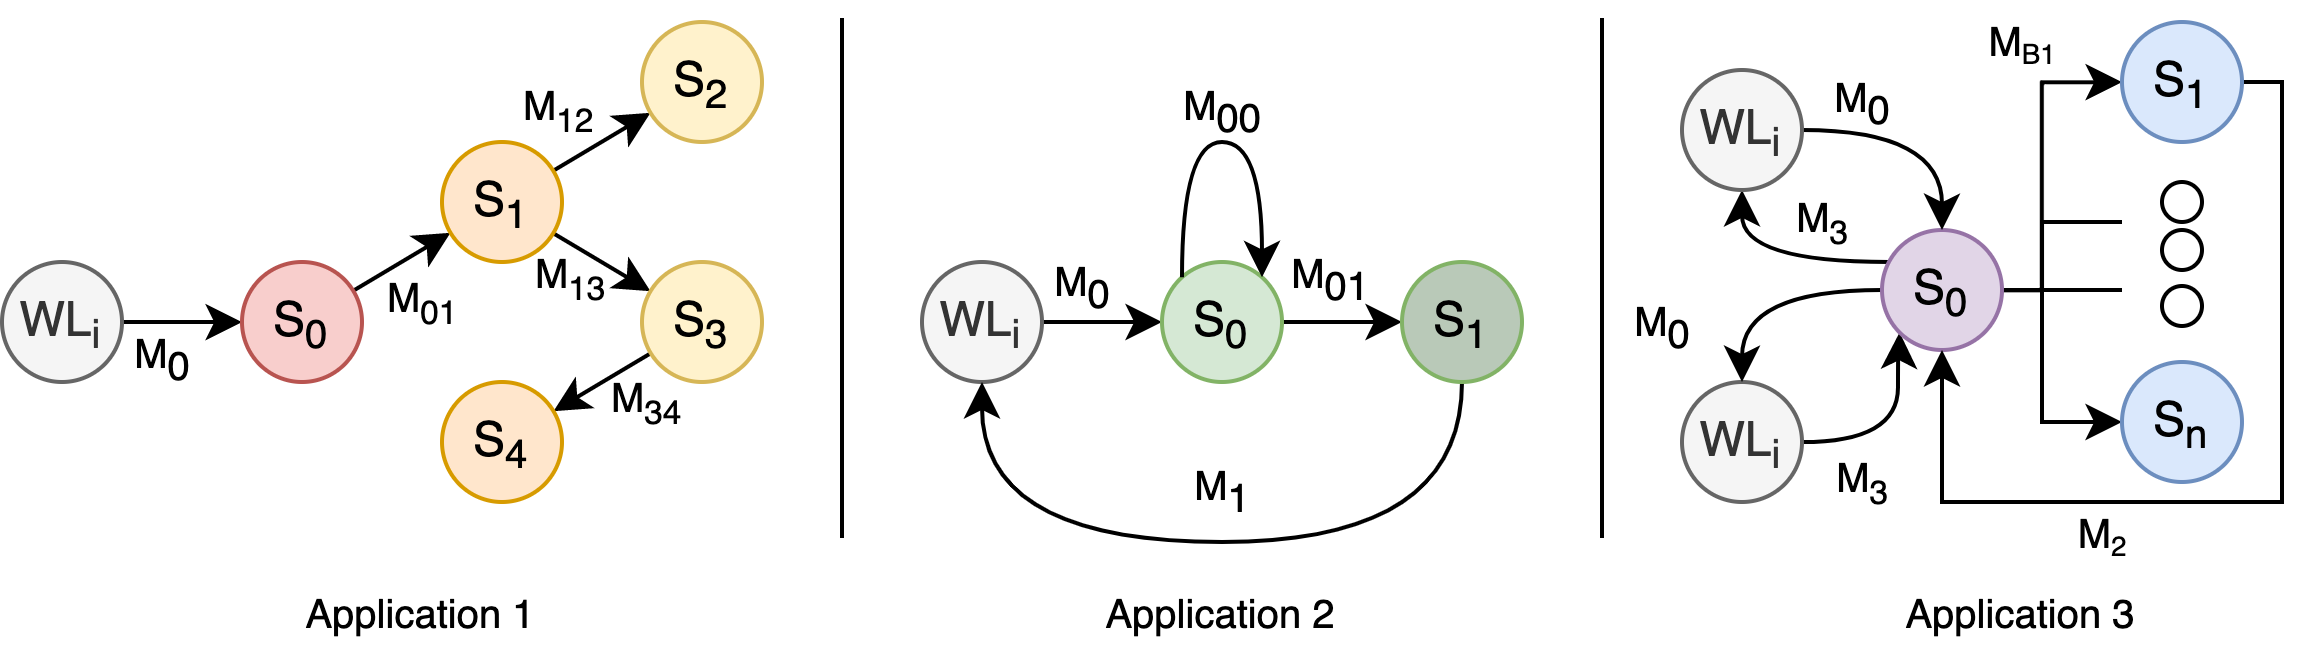
\includegraphics[width=14cm]{images/applications_ddf}
  \centering
  \caption{Tre tipologie di applicazioni realizzabili, con la loro rappresentazione tramite grafo.}
  \label{fig:applications_ddf}
\end{figure}

La definizione delle applicazioni è composta da quattro parti: \textit{moduli} (o \textit{servizi}), \textit{messaggi}, \textit{trasmissioni} e dati generali. I \textit{moduli} possono avere diversi attributi, anche a seconda dello specifico scenario, ma quelli obbligatori sono solo un identificativo univoco (\textit{ID}) e il nome (\textit{name}). I \textit{messaggi}, ovvero i dati scambiati, hanno principalmente due attributi obbligatori: il numero di istruzioni (\textit{instructions}) e la grandezza in byte (\textit{bytes}). Le \textit{trasmissioni} definiscono le modalità in cui i servizi scambiano le informazioni. Gli attributi obbligatori sono in questo caso: il modulo di appartenenza (\textit{module}) e il messaggio in ingresso. Tramite la definizione delle trasmissioni è possibile, tramite un particolare attributo detto \textit{fractional}, definire la probabilità di propagare un determinato messaggio \textit{message\_out} sulla ricezione di un particolare messaggio \textit{message\_in}. 

In Figura \ref{fig:applications_ddf} sono mostrate tre tipologie di applicazioni che sono realizzabili. La prima, \texttt{Application 1}, è strutturata gerarchicamente, con la ricezione dei messaggi $M_{ij}$ che scatena l'invio di altri messaggi. Nella seconda applicazione, \texttt{Application 2}, è possibile osservare un'interazione di un servizio con se stesso. Infine nell'ultima applicazione, \texttt{Application 3}, è mostrato il \textit{broadcasting} di un messaggio $M_{B1}$ che raggiunge tutti i moduli dell'applicazione. In tutte e tre le applicazioni $WL_i$ indica il nodo che genera il carico di lavoro (ad esempio un dispositivo IoT).


\section{Descrizione dello scenario simulato}


















